%TEX root = ./overwiew.tex

\documentclass{standalone}

\usepackage{tikz}
\usetikzlibrary{positioning}
\usetikzlibrary{shapes,arrows}


\begin{document}
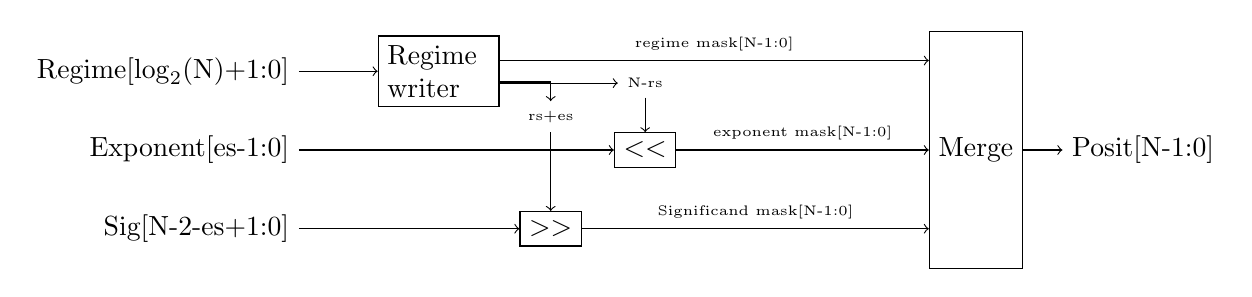
\begin{tikzpicture}
	\node (lc) {};
	\node (rc) [below right =2cm and 10cm of lc] {};

	\node (regime) [below=0cm of lc, left] {Regime[$\log_2$(N)+1:0]};
	\node (exp) [below=1cm of lc, left] {Exponent[es-1:0]};
	\node (sig) [below=2cm of lc, left] {Sig[N-2-es+1:0]};

	\node[draw] (merge) [right=8cm of exp, minimum height=3cm] {Merge};
	\node (output) [right=0.5cm of merge] {Posit[N-1:0]};

	\node[draw] (rwriter) [right=1cm of regime] {\parbox{1.3cm}{Regime writer}};
	\node[draw] (eswriter) [right=4cm of exp] {$<<$};
	\node (diff) [above=0.44cm of eswriter]{\tiny N-rs};

	\node[draw] (swriter) [right=2.8cm of sig] {$>>$};
	\node (esplus) [above=1cm of swriter] {\tiny rs+es};


	\path[draw, ->] (regime) -- (rwriter);
	\path[draw, ->] (rwriter.10) -- node[above, midway] {\tiny regime mask[N-1:0]} (rwriter.10 -| merge.180);

	\path[draw, ->] (exp) -- (eswriter);
	\path[draw, ->] (rwriter.-10) |- (diff);
	\path[draw, ->] (diff) -- (eswriter);
	\path[draw, ->] (eswriter) -- node[above, midway] {\tiny exponent mask[N-1:0]} (merge);

	\path[draw, ->] (sig) -- (swriter);
	\path[draw, ->] (swriter) -- node[above, midway] {\tiny Significand mask[N-1:0]} (merge.180 |- sig);
	\path[draw, ->] (rwriter.-10) -| (esplus);
	\path[draw, ->] (esplus) -- (swriter);

	\path[draw, ->] (merge) -- (output);

\end{tikzpicture}
\end{document}